\documentclass[a3paper,landscape]{article}

\usepackage[margin=0.30cm]{geometry}
\usepackage{tikz}
\usepackage{adjustbox}

\usetikzlibrary{arrows.meta,calc}

\pagestyle{empty}

% =========================================================
% ESTILOS
% =========================================================

\tikzset{
umlclass/.style={
    draw,
    rectangle,
    rounded corners=2pt,
    text width=4.45cm,
    align=left,
    inner sep=4pt,
    font=\scriptsize
},
umlinterface/.style={
    draw,
    rectangle,
    dashed,
    rounded corners=2pt,
    text width=4.45cm,
    align=left,
    inner sep=4pt,
    font=\scriptsize
},
umlabstract/.style={
    draw,
    rectangle,
    rounded corners=2pt,
    text width=4.45cm,
    align=left,
    inner sep=4pt,
    font=\scriptsize
},
umlwide/.style={
    draw,
    rectangle,
    rounded corners=2pt,
    text width=5.25cm,
    align=left,
    inner sep=4pt,
    font=\scriptsize
},
umlsmall/.style={
    draw,
    rectangle,
    rounded corners=2pt,
    text width=4.05cm,
    align=left,
    inner sep=4pt,
    font=\scriptsize
},
herencia/.style={
    thick,
    -{Triangle[open,length=3mm,width=3mm]}
},
implementa/.style={
    thick,
    dashed,
    -{Triangle[open,length=3mm,width=3mm]}
},
depende/.style={
    dashed,
    -{Stealth[length=2.5mm]}
},
asocia/.style={
    thick
}
}

% =========================================================
% DOCUMENTO
% =========================================================

\begin{document}

\begin{center}
{\Large\bfseries Diagrama de Clases -- Sistema de Gestion de Drones -- Composite y Adapter}
\end{center}

\vspace{0.05cm}

\begin{adjustbox}{
max width=\textwidth,
max totalheight=0.90\textheight,
center
}

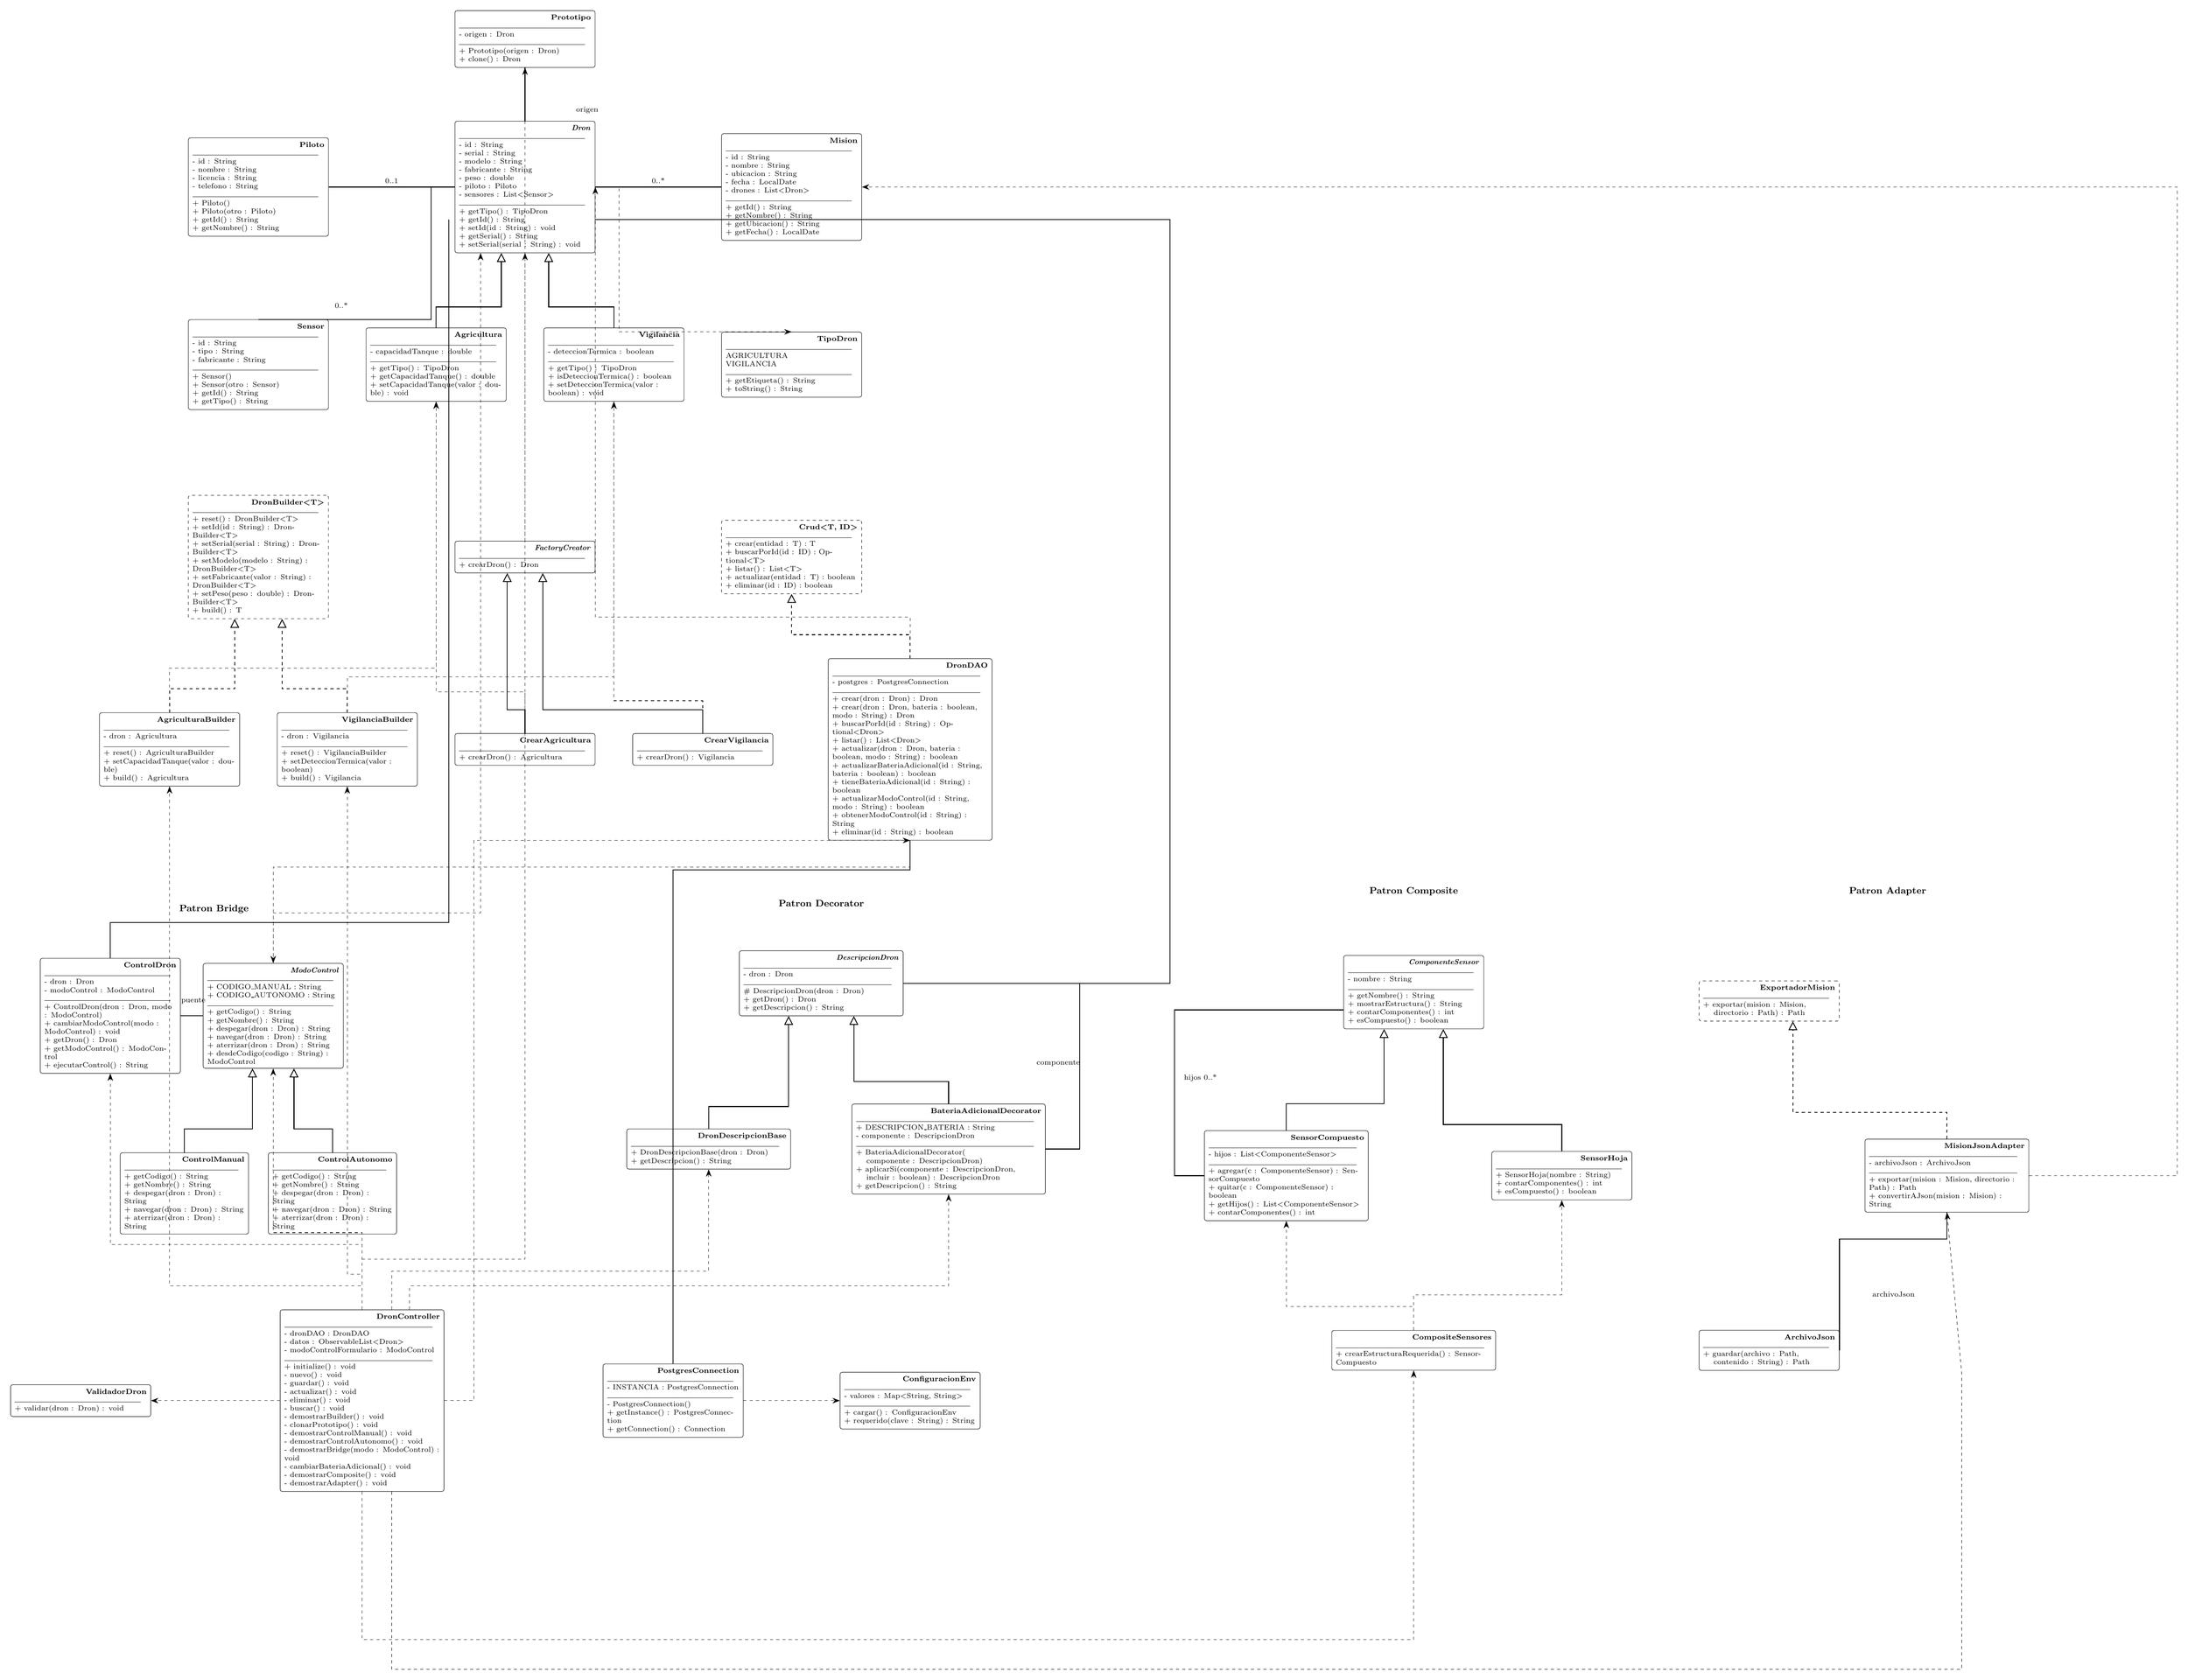
\begin{tikzpicture}

% =========================================================
% FILA 1 - PROTOTYPE
% =========================================================

\node[umlclass] (Prototipo) at (0,19) {
\textbf{\hfill Prototipo\hfill}\\
\rule{4.25cm}{0.3pt}\\
- origen : Dron\\
\rule{4.25cm}{0.3pt}\\
+ Prototipo(origen : Dron)\\
+ clone() : Dron
};

% =========================================================
% FILA 2 - MODELO PRINCIPAL
% El package modelo permanece sin modificaciones.
% =========================================================

\node[umlclass] (Piloto) at (-9,14) {
\textbf{\hfill Piloto\hfill}\\
\rule{4.25cm}{0.3pt}\\
- id : String\\
- nombre : String\\
- licencia : String\\
- telefono : String\\
\rule{4.25cm}{0.3pt}\\
+ Piloto()\\
+ Piloto(otro : Piloto)\\
+ getId() : String\\
+ getNombre() : String
};

\node[umlabstract] (Dron) at (0,14) {
\textbf{\hfill \textit{Dron}\hfill}\\
\rule{4.25cm}{0.3pt}\\
- id : String\\
- serial : String\\
- modelo : String\\
- fabricante : String\\
- peso : double\\
- piloto : Piloto\\
- sensores : List\textless Sensor\textgreater\\
\rule{4.25cm}{0.3pt}\\
+ getTipo() : TipoDron\\
+ getId() : String\\
+ setId(id : String) : void\\
+ getSerial() : String\\
+ setSerial(serial : String) : void
};

\node[umlclass] (Mision) at (9,14) {
\textbf{\hfill Mision\hfill}\\
\rule{4.25cm}{0.3pt}\\
- id : String\\
- nombre : String\\
- ubicacion : String\\
- fecha : LocalDate\\
- drones : List\textless Dron\textgreater\\
\rule{4.25cm}{0.3pt}\\
+ getId() : String\\
+ getNombre() : String\\
+ getUbicacion() : String\\
+ getFecha() : LocalDate
};

% =========================================================
% FILA 3 - SUBCLASES DEL MODELO
% =========================================================

\node[umlclass] (Sensor) at (-9,8) {
\textbf{\hfill Sensor\hfill}\\
\rule{4.25cm}{0.3pt}\\
- id : String\\
- tipo : String\\
- fabricante : String\\
\rule{4.25cm}{0.3pt}\\
+ Sensor()\\
+ Sensor(otro : Sensor)\\
+ getId() : String\\
+ getTipo() : String
};

\node[umlclass] (Agricultura) at (-3,8) {
\textbf{\hfill Agricultura\hfill}\\
\rule{4.25cm}{0.3pt}\\
- capacidadTanque : double\\
\rule{4.25cm}{0.3pt}\\
+ getTipo() : TipoDron\\
+ getCapacidadTanque() : double\\
+ setCapacidadTanque(valor : double) : void
};

\node[umlclass] (Vigilancia) at (3,8) {
\textbf{\hfill Vigilancia\hfill}\\
\rule{4.25cm}{0.3pt}\\
- deteccionTermica : boolean\\
\rule{4.25cm}{0.3pt}\\
+ getTipo() : TipoDron\\
+ isDeteccionTermica() : boolean\\
+ setDeteccionTermica(valor : boolean) : void
};

\node[umlclass] (TipoDron) at (9,8) {
\textbf{\hfill TipoDron\hfill}\\
\rule{4.25cm}{0.3pt}\\
AGRICULTURA\\
VIGILANCIA\\
\rule{4.25cm}{0.3pt}\\
+ getEtiqueta() : String\\
+ toString() : String
};

% =========================================================
% FILA 4 - BUILDER / FACTORY / CRUD
% =========================================================

\node[umlinterface] (DronBuilder) at (-9,1.5) {
\textbf{\hfill DronBuilder\textless T\textgreater\hfill}\\
\rule{4.25cm}{0.3pt}\\
+ reset() : DronBuilder\textless T\textgreater\\
+ setId(id : String) : DronBuilder\textless T\textgreater\\
+ setSerial(serial : String) : DronBuilder\textless T\textgreater\\
+ setModelo(modelo : String) : DronBuilder\textless T\textgreater\\
+ setFabricante(valor : String) : DronBuilder\textless T\textgreater\\
+ setPeso(peso : double) : DronBuilder\textless T\textgreater\\
+ build() : T
};

\node[umlabstract] (FactoryCreator) at (0,1.5) {
\textbf{\hfill \textit{FactoryCreator}\hfill}\\
\rule{4.25cm}{0.3pt}\\
+ crearDron() : Dron
};

\node[umlinterface] (Crud) at (9,1.5) {
\textbf{\hfill Crud\textless T, ID\textgreater\hfill}\\
\rule{4.25cm}{0.3pt}\\
+ crear(entidad : T) : T\\
+ buscarPorId(id : ID) : Optional\textless T\textgreater\\
+ listar() : List\textless T\textgreater\\
+ actualizar(entidad : T) : boolean\\
+ eliminar(id : ID) : boolean
};

% =========================================================
% FILA 5 - BUILDER / FACTORY / DAO
% =========================================================

\node[umlclass] (AgrBuilder) at (-12,-5) {
\textbf{\hfill AgriculturaBuilder\hfill}\\
\rule{4.25cm}{0.3pt}\\
- dron : Agricultura\\
\rule{4.25cm}{0.3pt}\\
+ reset() : AgriculturaBuilder\\
+ setCapacidadTanque(valor : double)\\
+ build() : Agricultura
};

\node[umlclass] (VigBuilder) at (-6,-5) {
\textbf{\hfill VigilanciaBuilder\hfill}\\
\rule{4.25cm}{0.3pt}\\
- dron : Vigilancia\\
\rule{4.25cm}{0.3pt}\\
+ reset() : VigilanciaBuilder\\
+ setDeteccionTermica(valor : boolean)\\
+ build() : Vigilancia
};

\node[umlclass] (CrearAgricultura) at (0,-5) {
\textbf{\hfill CrearAgricultura\hfill}\\
\rule{4.25cm}{0.3pt}\\
+ crearDron() : Agricultura
};

\node[umlclass] (CrearVigilancia) at (6,-5) {
\textbf{\hfill CrearVigilancia\hfill}\\
\rule{4.25cm}{0.3pt}\\
+ crearDron() : Vigilancia
};

\node[umlwide] (DronDAO) at (13,-5) {
\textbf{\hfill DronDAO\hfill}\\
\rule{5.0cm}{0.3pt}\\
- postgres : PostgresConnection\\
\rule{5.0cm}{0.3pt}\\
+ crear(dron : Dron) : Dron\\
+ crear(dron : Dron, bateria : boolean, modo : String) : Dron\\
+ buscarPorId(id : String) : Optional\textless Dron\textgreater\\
+ listar() : List\textless Dron\textgreater\\
+ actualizar(dron : Dron, bateria : boolean, modo : String) : boolean\\
+ actualizarBateriaAdicional(id : String, bateria : boolean) : boolean\\
+ tieneBateriaAdicional(id : String) : boolean\\
+ actualizarModoControl(id : String, modo : String) : boolean\\
+ obtenerModoControl(id : String) : String\\
+ eliminar(id : String) : boolean
};

% =========================================================
% FILA 6 - BRIDGE
% =========================================================

\node at (-10.5,-10.4) {
\textbf{\small Patron Bridge}
};

\node[umlclass] (ControlDron) at (-14,-14) {
\textbf{\hfill ControlDron\hfill}\\
\rule{4.25cm}{0.3pt}\\
- dron : Dron\\
- modoControl : ModoControl\\
\rule{4.25cm}{0.3pt}\\
+ ControlDron(dron : Dron, modo : ModoControl)\\
+ cambiarModoControl(modo : ModoControl) : void\\
+ getDron() : Dron\\
+ getModoControl() : ModoControl\\
+ ejecutarControl() : String
};

\node[umlabstract] (ModoControl) at (-8.5,-14) {
\textbf{\hfill \textit{ModoControl}\hfill}\\
\rule{4.25cm}{0.3pt}\\
+ CODIGO\_MANUAL : String\\
+ CODIGO\_AUTONOMO : String\\
\rule{4.25cm}{0.3pt}\\
+ getCodigo() : String\\
+ getNombre() : String\\
+ despegar(dron : Dron) : String\\
+ navegar(dron : Dron) : String\\
+ aterrizar(dron : Dron) : String\\
+ desdeCodigo(codigo : String) : ModoControl
};

\node[umlsmall] (ControlManual) at (-11.5,-20) {
\textbf{\hfill ControlManual\hfill}\\
\rule{3.85cm}{0.3pt}\\
+ getCodigo() : String\\
+ getNombre() : String\\
+ despegar(dron : Dron) : String\\
+ navegar(dron : Dron) : String\\
+ aterrizar(dron : Dron) : String
};

\node[umlsmall] (ControlAutonomo) at (-6.5,-20) {
\textbf{\hfill ControlAutonomo\hfill}\\
\rule{3.85cm}{0.3pt}\\
+ getCodigo() : String\\
+ getNombre() : String\\
+ despegar(dron : Dron) : String\\
+ navegar(dron : Dron) : String\\
+ aterrizar(dron : Dron) : String
};

% =========================================================
% FILA 6 - DECORATOR
% Disposicion vertical para evitar cruces y texto sobrepuesto
% =========================================================

\node at (10,-10.2) {
\textbf{\small Patron Decorator}
};

% Clase abstracta en la parte superior
\node[umlwide] (DescripcionDron) at (10,-12.9) {
\textbf{\hfill \textit{DescripcionDron}\hfill}\\
\rule{5.0cm}{0.3pt}\\
- dron : Dron\\
\rule{5.0cm}{0.3pt}\\
\# DescripcionDron(dron : Dron)\\
+ getDron() : Dron\\
+ getDescripcion() : String
};

% Subclase base, separada a la izquierda
\node[umlwide] (DronDescripcionBase) at (6.2,-18.5) {
\textbf{\hfill DronDescripcionBase\hfill}\\
\rule{5.0cm}{0.3pt}\\
+ DronDescripcionBase(dron : Dron)\\
+ getDescripcion() : String
};

% Decorador concreto, con mayor ancho y saltos de linea controlados
\node[umlwide, text width=6.25cm] (BateriaAdicionalDecorator) at (14.3,-18.5) {
\textbf{\hfill BateriaAdicionalDecorator\hfill}\\
\rule{6.0cm}{0.3pt}\\
+ DESCRIPCION\_BATERIA : String\\
- componente : DescripcionDron\\
\rule{6.0cm}{0.3pt}\\
+ BateriaAdicionalDecorator(\\
\hspace{0.35cm}componente : DescripcionDron)\\
+ aplicarSi(componente : DescripcionDron,\\
\hspace{0.35cm}incluir : boolean) : DescripcionDron\\
+ getDescripcion() : String
};

% =========================================================
% FILA 7 - SERVICIOS / CONTROLADOR / SINGLETON
% =========================================================

\node[umlclass] (ValidadorDron) at (-15,-27) {
\textbf{\hfill ValidadorDron\hfill}\\
\rule{4.25cm}{0.3pt}\\
+ validar(dron : Dron) : void
};

\node[umlwide] (DronController) at (-5.5,-27) {
\textbf{\hfill DronController\hfill}\\
\rule{5.0cm}{0.3pt}\\
- dronDAO : DronDAO\\
- datos : ObservableList\textless Dron\textgreater\\
- modoControlFormulario : ModoControl\\
\rule{5.0cm}{0.3pt}\\
+ initialize() : void\\
- nuevo() : void\\
- guardar() : void\\
- actualizar() : void\\
- eliminar() : void\\
- buscar() : void\\
- demostrarBuilder() : void\\
- clonarPrototipo() : void\\
- demostrarControlManual() : void\\
- demostrarControlAutonomo() : void\\
- demostrarBridge(modo : ModoControl) : void\\
- cambiarBateriaAdicional() : void\\
- demostrarComposite() : void\\
- demostrarAdapter() : void
};

\node[umlclass] (PostgresConnection) at (5,-27) {
\textbf{\hfill PostgresConnection\hfill}\\
\rule{4.25cm}{0.3pt}\\
- INSTANCIA : PostgresConnection\\
\rule{4.25cm}{0.3pt}\\
- PostgresConnection()\\
+ getInstance() : PostgresConnection\\
+ getConnection() : Connection
};

\node[umlclass] (ConfiguracionEnv) at (13,-27) {
\textbf{\hfill ConfiguracionEnv\hfill}\\
\rule{4.25cm}{0.3pt}\\
- valores : Map\textless String, String\textgreater\\
\rule{4.25cm}{0.3pt}\\
+ cargar() : ConfiguracionEnv\\
+ requerido(clave : String) : String
};



% =========================================================
% COLUMNA DERECHA - COMPOSITE
% Se ubica fuera del bloque existente para evitar sobreposiciones.
% =========================================================

\node at (30,-9.8) {
\textbf{\small Patron Composite}
};

\node[umlabstract] (ComponenteSensor) at (30,-13.2) {
\textbf{\hfill \textit{ComponenteSensor}\hfill}\\
\rule{4.25cm}{0.3pt}\\
- nombre : String\\
\rule{4.25cm}{0.3pt}\\
+ getNombre() : String\\
+ mostrarEstructura() : String\\
+ contarComponentes() : int\\
+ esCompuesto() : boolean
};

\node[umlwide] (SensorCompuesto) at (25.7,-19.4) {
\textbf{\hfill SensorCompuesto\hfill}\\
\rule{5.0cm}{0.3pt}\\
- hijos : List\textless ComponenteSensor\textgreater\\
\rule{5.0cm}{0.3pt}\\
+ agregar(c : ComponenteSensor) : SensorCompuesto\\
+ quitar(c : ComponenteSensor) : boolean\\
+ getHijos() : List\textless ComponenteSensor\textgreater\\
+ contarComponentes() : int
};

\node[umlclass] (SensorHoja) at (35.0,-19.4) {
\textbf{\hfill SensorHoja\hfill}\\
\rule{4.25cm}{0.3pt}\\
+ SensorHoja(nombre : String)\\
+ contarComponentes() : int\\
+ esCompuesto() : boolean
};

\node[umlwide] (CompositeSensores) at (30,-25.3) {
\textbf{\hfill CompositeSensores\hfill}\\
\rule{5.0cm}{0.3pt}\\
+ crearEstructuraRequerida() : SensorCompuesto
};

% =========================================================
% COLUMNA DERECHA - ADAPTER
% =========================================================

\node at (46,-9.8) {
\textbf{\small Patron Adapter}
};

\node[umlinterface] (ExportadorMision) at (42,-13.5) {
\textbf{\hfill ExportadorMision\hfill}\\
\rule{4.25cm}{0.3pt}\\
+ exportar(mision : Mision,\\
\hspace{0.35cm}directorio : Path) : Path
};

\node[umlwide] (MisionJsonAdapter) at (48,-19.4) {
\textbf{\hfill MisionJsonAdapter\hfill}\\
\rule{5.0cm}{0.3pt}\\
- archivoJson : ArchivoJson\\
\rule{5.0cm}{0.3pt}\\
+ exportar(mision : Mision, directorio : Path) : Path\\
+ convertirAJson(mision : Mision) : String
};

\node[umlclass] (ArchivoJson) at (42,-25.3) {
\textbf{\hfill ArchivoJson\hfill}\\
\rule{4.25cm}{0.3pt}\\
+ guardar(archivo : Path,\\
\hspace{0.35cm}contenido : String) : Path
};

% =========================================================
% RELACIONES PROTOTYPE
% =========================================================

\draw[asocia]
(Prototipo.south)
--
(Dron.north);

\node at (2.1,16.6) {\scriptsize origen};

% =========================================================
% HERENCIA DE DRON
% =========================================================

\draw[herencia]
(Agricultura.north)
-- ++(0,0.7)
-| ($(Dron.south)+(-0.8,0)$);

\draw[herencia]
(Vigilancia.north)
-- ++(0,0.7)
-| ($(Dron.south)+(0.8,0)$);

% =========================================================
% RELACIONES DEL MODELO
% =========================================================

\draw[asocia]
(Dron.west)
--
node[above]{\scriptsize 0..1}
(Piloto.east);

\draw[asocia]
(Dron.west)
-- ++(-0.8,0)
|- (Sensor.north);

\node at (-6.2,10) {\scriptsize 0..*};

\draw[asocia]
(Mision.west)
--
node[above]{\scriptsize 0..*}
(Dron.east);

\draw[depende]
(Dron.east)
-- ++(0.8,0)
|- (TipoDron.north);

% =========================================================
% BUILDER
% =========================================================

\draw[implementa]
(AgrBuilder.north)
-- ++(0,0.8)
-| ($(DronBuilder.south)+(-0.8,0)$);

\draw[implementa]
(VigBuilder.north)
-- ++(0,0.8)
-| ($(DronBuilder.south)+(0.8,0)$);

\draw[depende]
(AgrBuilder.north)
-- ++(0,1.5)
-| (Agricultura.south);

\draw[depende]
(VigBuilder.north)
-- ++(0,1.2)
-| (Vigilancia.south);

% =========================================================
% FACTORY METHOD
% =========================================================

\draw[herencia]
(CrearAgricultura.north)
-- ++(0,0.8)
-| ($(FactoryCreator.south)+(-0.6,0)$);

\draw[herencia]
(CrearVigilancia.north)
-- ++(0,0.8)
-| ($(FactoryCreator.south)+(0.6,0)$);

\draw[depende]
(CrearAgricultura.north)
-- ++(0,1.4)
-| (Agricultura.south);

\draw[depende]
(CrearVigilancia.north)
-- ++(0,1.1)
-| (Vigilancia.south);

\draw[depende]
(FactoryCreator.north)
--
(Dron.south);

% =========================================================
% DAO
% =========================================================

\draw[implementa]
(DronDAO.north)
-- ++(0,0.8)
-| (Crud.south);

\draw[depende]
(DronDAO.north)
-- ++(0,1.4)
-| (Dron.east);

\draw[asocia]
(DronDAO.south)
-- ++(0,-1)
-| (PostgresConnection.north);

% DronDAO usa los codigos de ModoControl para persistir Bridge.
% La linea se enruta por una franja libre entre DAO y los patrones.
\draw[depende]
(DronDAO.south)
-- ++(0,-0.9)
-- ++(-21.5,0)
-- (ModoControl.north);

% =========================================================
% BRIDGE
% =========================================================

% ControlDron mantiene el puente hacia ModoControl
\draw[asocia]
(ControlDron.east)
--
(ModoControl.west);

\node at (-11.2,-13.5) {\scriptsize puente};

% ControlDron contiene el Dron real
\draw[asocia]
(ControlDron.north)
-- ++(0,1.2)
-| ($(Dron.west)+(-0.2,-1.1)$);

% ModoControl opera sobre Dron
\draw[depende]
(ModoControl.north)
-- ++(0,1.7)
-| ($(Dron.south)+(-1.5,0)$);

% Dos subclases reales de Bridge
\draw[herencia]
(ControlManual.north)
-- ++(0,0.8)
-| ($(ModoControl.south)+(-0.7,0)$);

\draw[herencia]
(ControlAutonomo.north)
-- ++(0,0.8)
-| ($(ModoControl.south)+(0.7,0)$);

% =========================================================
% DECORATOR
% =========================================================

% Herencia: las flechas llegan por debajo de la clase abstracta,
% sin atravesar el contenido de los nodos.
\draw[herencia]
(DronDescripcionBase.north)
-- ++(0,0.75)
-| ($(DescripcionDron.south)+(-1.1,0)$);

\draw[herencia]
(BateriaAdicionalDecorator.north)
-- ++(0,0.75)
-| ($(DescripcionDron.south)+(1.1,0)$);

% Composicion del Decorator: se enruta por el costado derecho
% para no cruzar la herencia ni atravesar otras clases.
\draw[asocia]
(BateriaAdicionalDecorator.east)
-- ++(1.15,0)
|- (DescripcionDron.east);

\node at (18.0,-15.6) {\scriptsize componente};

% Relacion con Dron: se lleva por el borde exterior derecho.
\draw[asocia]
(DescripcionDron.east)
-- ++(9.0,0)
|- ($(Dron.east)+(0,-1.1)$);

% =========================================================
% CONFIGURACION
% =========================================================

\draw[depende]
(PostgresConnection.east)
--
(ConfiguracionEnv.west);

% =========================================================
% CONTROLADOR
% =========================================================

\draw[depende]
(DronController.west)
--
(ValidadorDron.east);

% Controlador utiliza DAO concreto
\draw[depende]
(DronController.east)
-- ++(1.0,0)
|- (DronDAO.south);

% Controlador utiliza Builder
\draw[depende]
(DronController.north)
-- ++(0,0.8)
-| (AgrBuilder.south);

\draw[depende]
(DronController.north)
-- ++(0,1.2)
-| (VigBuilder.south);

% Controlador utiliza Prototype como servicio
\draw[depende]
(DronController.north)
-- ++(0,1.7)
-| (Prototipo.south);

% Controlador utiliza Bridge
\draw[depende]
(DronController.north)
-- ++(0,2.2)
-| (ControlDron.south);

\draw[depende]
(DronController.north)
-- ++(0,2.6)
-| (ModoControl.south);

% Controlador utiliza Decorator.
% Las dependencias salen por la parte superior del controlador y
% recorren una franja libre por debajo de las subclases.
\draw[depende]
($(DronController.north)+(1.0,0)$)
-- ++(0,1.3)
-| (DronDescripcionBase.south);

\draw[depende]
($(DronController.north)+(1.6,0)$)
-- ++(0,0.8)
-| (BateriaAdicionalDecorator.south);



% =========================================================
% COMPOSITE
% =========================================================

% Las dos clases concretas comparten el mismo componente abstracto.
\draw[herencia]
(SensorCompuesto.north)
-- ++(0,0.9)
-| ($(ComponenteSensor.south)+(-1.0,0)$);

\draw[herencia]
(SensorHoja.north)
-- ++(0,0.9)
-| ($(ComponenteSensor.south)+(1.0,0)$);

% El Composite contiene cero o mas componentes del mismo tipo comun.
\draw[asocia]
(SensorCompuesto.west)
-- ++(-1.0,0)
|- ($(ComponenteSensor.west)+(0,-0.6)$);

\node at (22.8,-16.1) {\scriptsize hijos 0..*};

% La clase de apoyo construye tanto nodos compuestos como hojas.
\draw[depende]
(CompositeSensores.north)
-- ++(0,0.8)
-| (SensorCompuesto.south);

\draw[depende]
(CompositeSensores.north)
-- ++(0,1.2)
-| (SensorHoja.south);

% =========================================================
% ADAPTER
% =========================================================

% El Adapter implementa el Target.
\draw[implementa]
(MisionJsonAdapter.north)
-- ++(0,0.9)
-| ($(ExportadorMision.south)+(0.8,0)$);

% El Adapter delega la escritura fisica al Adaptee.
\draw[asocia]
(MisionJsonAdapter.south)
-- ++(0,-0.9)
-| (ArchivoJson.east);

\node at (46.2,-23.4) {\scriptsize archivoJson};

% El Adapter recibe una instancia de Mision sin modificar el modelo.
\draw[depende]
(MisionJsonAdapter.east)
-- ++(5.0,0)
-- ++(0,33.4)
-- ++(-39.0,0)
-- (Mision.east);

% =========================================================
% CONTROLADOR - NUEVOS PATRONES
% =========================================================

% Las nuevas dependencias se enrutan por debajo del bloque principal.
\draw[depende]
(DronController.south)
-- ++(0,-5.0)
-- ++(35.5,0)
-- (CompositeSensores.south);

\draw[depende]
($(DronController.south)+(1.0,0)$)
-- ++(0,-6.0)
-- ++(53.0,0)
-- ++(0,10.0)
-- (MisionJsonAdapter.south);

\end{tikzpicture}

\end{adjustbox}

\end{document}
